%\documentclass[12pt,a4paper]{report}
%\usepackage[utf8]{inputenc}
%\usepackage{amsmath}
%\usepackage{amsfonts}
%\usepackage{amssymb}
%\usepackage[margin=2.5cm]{geometry}
%\usepackage{graphicx}
%\usepackage{caption}
%\usepackage{subcaption}
%\usepackage[nottoc,numbib]{tocbibind}
%\linespread{1.3}
%\begin{document}
	\chapter{Appendix}
	\label{Appendix}
%%%%%
%%%%%
%%%%%
%%%%%
%%%%%
	\section{Quantum Harmonic Oscillator}
	\label{Appendix - Quantum Harmonic Oscillator}
		For a free particle with a mass $m$, the time independent Schr{\" o}dinger equation in one spacial dimension takes the form of:
		\begin{equation}
			\hat{H}\psi=E\psi
		\end{equation}
		where:
		\begin{equation}
			\hat{H}=\frac{\hat{p}}{2m}+V\left(x\right)
		\end{equation}
		With the potential \cite{b33}:
		\begin{equation}
			V\left(x\right)=\frac{1}{2}m\omega^{2}x^{2}
		\end{equation}
		the Schr{\" o}dinger equation can be expressed as:
		\begin{equation}
			\left[-\frac{\partial^{2}}{\partial x^{2}}+\alpha^{2}x^{2}\right]\psi=\frac{2m}{\hbar^{2}}E\psi
			\label{QHO}
		\end{equation}
		where $\alpha=m\omega/\hbar$. This equation has the solution:
		\begin{equation}
			\psi_{n}=\left(\frac{\alpha}{\pi}\right)^{\frac{1}{4}}\frac{1}{\sqrt{2^{n}n!}}H_{n}\left(\sqrt{\alpha}x\right)e^{-\frac{\alpha}{2}x^{2}}
		\end{equation}
		Where $H_{n}\left(x\right)$ is the Hermite polynomial:
		\begin{equation}
			H_{n}\left(x\right)=\left(-1\right)^{n}e^{x^{n}}\frac{d^{n}}{dx^{n}}e^{-x^{n}}
		\end{equation}
		The Hermite polynomials for the first three values of $n$ are:
		\begin{align}
			H_{0}\left(x\right)&=1\\
			H_{1}\left(x\right)&=2x\\
			H_{2}\left(x\right)&=4x^{2}-2
		\end{align}
		Therefore the wave-functions for the first three energy levels become:
		\begin{align}
			\psi_{0}&=\left(\frac{\alpha}{\pi}\right)^{\frac{1}{4}}e^{-\frac{\alpha}{2}x^{2}}\\
			\psi_{1}&=\left(\frac{\alpha}{\pi}\right)^{\frac{1}{4}}\sqrt{2\alpha}xe^{-\frac{\alpha}{2}x^{2}}\\
			\psi_{2}&=\left(\frac{\alpha}{\pi}\right)^{\frac{1}{4}}\frac{1}{\sqrt{2}}\left(2\alpha x^2-1\right)e^{-\frac{\alpha}{2}x^{2}}
		\end{align}
		Using these wave-functions in Equation (\ref{QHO}) produces the first three energy levels:
		\begin{align}
			E_{0}&=\frac{\hbar\omega}{2}\\
			E_{1}&=\frac{3}{2}\hbar\omega\\
			E_{2}&=\frac{5}{2}\hbar\omega
		\end{align}
		With these energy levels the expression for energy can be generalised to:
		\begin{equation}
			E_{n}=\hbar\omega\left(n+\frac{1}{2}\right)
		\end{equation}
%%%%%
%%%%%
%%%%%
%%%%%
%%%%%
	\section{Evaluating $p_{z}$}
	\label{Appendix - pz}
		To evaluate the expression:
		\begin{equation}
			\frac{1}{1-\hat{p}_{z}}e^{ik_{z}z}
		\end{equation}
		use the Taylor expansion:
		\begin{align}
			\frac{1}{1-\hat{p}_{z}}e^{ik_{z}z}&=\left(1+\hat{p}_{z}+\hat{p}_{z}^{2}+...\right)e^{ik_{z}z}\\
			&=\left(1-i\hbar\frac{\partial}{\partial z}-\hbar^{2}\frac{\partial^{2}}{\partial z^{2}}+...\right)e^{ik_{z}z}\\
			&=\left(1+\hbar k_{z}+\hbar^{2}k_{z}^{2}+...\right)e^{ik_{z}z}
		\end{align}
		From this the relation:
		\begin{equation}
			\hat{p}_{z}=\hbar k_{z}
		\end{equation}
		can be made, which results in:
		\begin{equation}
			\frac{1}{1-\hat{p}_{z}}e^{ik_{z}z}=\frac{1}{1-\hbar k_{z}}e^{ik_{z}z}
		\end{equation}
%%%%%
%%%%%
%%%%%
%%%%%
%%%%%
	\section{Schr{\" o}dinger WKB Barrier}
	\label{Appendix - Schrodinger WKB Barrier}
		The scattering properties of the Schr{\" o}dinger smooth potential will derived in this section. This will be used as a comparison for the graphene case.
		\subsection{Defining the Schr{\" o}dinger System}
		\label{Appendix - Defining the Schrodinger System}
		\begin{figure}[h]
			\centerline{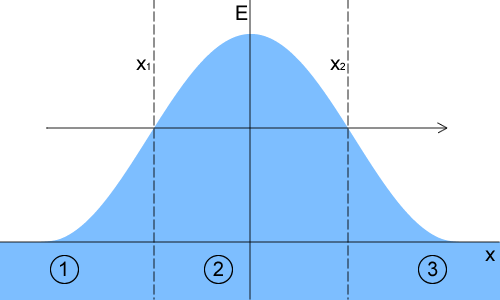
\includegraphics[scale=0.6]{images/s-wkb-potential-flat}}
			\caption{Diagram showing a smooth potential barrier for an arbitrary potential $V\left(x\right)$. The two turning points $x_{1,2}$ and the three independent barrier regions have been labelled.}
			\label{s-wkb-potential-flat}
		\end{figure}
		Starting with the Schr{\" o}dinger equation:
		\begin{equation}
			\hat{H}y\left(x\right)=Ey\left(x\right)
		\end{equation}
		with the Hamiltonian:
		\begin{equation}
			\hat{H}=\frac{\hat{p}^2}{2m_{e}}+V\left(x\right)
		\end{equation}
		and the substitutions:
		\begin{align}
			h=\frac{\hbar}{\sqrt{2m_{e}}}
			\hspace{1cm}
			q\left(x\right)=E-V\left(x\right)
		\end{align}
		the Schr{\" o}dinger equation can take the form:
		\begin{equation}
			h^{2}y''\left(x\right)+q\left(x\right)y\left(x\right)=0
		\end{equation}
		where $h$ is the small parameter and prime denotes differentiation with respect to $x$. Here we will introduce the variables, and remove the function notations for convenience:
		\begin{equation}
			z=z\left(x\right)\hspace{1cm}\varphi\left(z\right)=\sqrt{z'}y\left(x\right)
		\end{equation}
		With the Schr{\" o}dinger equation in this form and the definitions of $z$ and $\varphi$, the equation:
		\begin{equation}
			h^{2}\varphi''+\varphi\left(\Delta-R\left(z\right)\right)=0
			\label{varphi}
		\end{equation}
		will now be considered with $\Delta$ as a constant and $R\left(x\right)$ as an arbitrary function to be defined properly later. This equation can be expressed in terms of $y$:
		\begin{equation}
			h^{2}z'^{2}y''+h^{2}z'z''y'+h^{2}my+z'^{2}y\left(\Delta-R\left(z\right)\right)=0
		\end{equation}
		with:
		\begin{equation}
			m=\frac{1}{2}z'z'''-\frac{1}{4}z''^{2}
		\end{equation}
		The terms containing $h^{2}$ shall be considered as too small, therefore $h^{2}\rightarrow0$ and the two equations in terms of $y$ can be used to find $z$ in terms of $q(x)$:
		\begin{align}
			h^{2}z'^{2}y''+h^{2}z'z''y'+h^{2}my+z'^{2}y\left(\Delta-R\left(z\right)\right)&=h^{2}y''+q\left(x\right)y\\
			z'^{2}\left(\Delta-R\left(z\right)\right)&=q\left(x\right)
		\end{align}
		For the case where $\Delta=1$ and $R\left(z\right)=0$ these equations show that:
		\begin{align}
			z'^{2}&=q\left(x\right)\\
			z&=\int \sqrt{\pm q} dx
		\end{align}
%%%%%
%%%%%
%%%%%
%%%%%
%%%%%
		\subsection{Wave-functions Far From the Turning Points}
		\label{Appendix - Wave-functions Far From the Turning Points}
		Far from the turning points Equation (\ref{varphi}) may be used with $\Delta=1$ and $R\left(z\right)=0$. The general solution of $h^{2}\varphi''+\varphi=0$:
		\begin{equation}
			\varphi=e^{\frac{i}{h}z}
		\end{equation}
		can be expressed in terms of $y$ with a reflected component:
		\begin{align}
			y=\frac{1}{\sqrt{z'}}\left(c_{1}e^{\frac{i}{h}z}+c_{2}e^{-\frac{i}{h}z}\right)
		\end{align}
		with a substitution of values for $z$ the wave-functions far from the turning points are of the form:
		\begin{align}
			y_{1}&= q^{-\frac{1}{4}}\left(a_{1}e^{\frac{i}{h}\int_{x_{1}}^x \sqrt{q} dx}+a_{2}e^{-\frac{i}{h}\int_{x_{1}}^x \sqrt{q} dx}\right)\\
			y_{2}&= \left(-q\right)^{-\frac{1}{4}}\left(c_{1}e^{\frac{1}{h}\int_{x_{1}}^x \sqrt{-q}dx}+c_{2}e^{-\frac{1}{h}\int_{x_{1}}^x \sqrt{-q}dx}\right)\\
			y_{3}&= q^{-\frac{1}{4}}\left(d_{1}e^{\frac{i}{h}\int_{x_{2}}^x \sqrt{q} dx}+d_{2}e^{-\frac{i}{h}\int_{x_{2}}^x \sqrt{q} dx}\right)
		\end{align}
%%%%%
%%%%%
%%%%%
%%%%%
%%%%%
		\subsection{Wave-functions Close to the Turning Points}
		\label{Appendix - Wave-functions Close to the Turning Points}
		For wave-functions close to the turning points Equation (\ref{varphi}) can be used with $\Delta=0$ and $R\left(z\right)=z$, the general solution becomes:
		\begin{equation}
			y=\frac{h^{\frac{1}{6}}}{\sqrt{z'}}\left(k_{3}A_{i}\left(\frac{z}{h^{\frac{2}{3}}}\right)+k_{4}B_{i}\left(\frac{z}{h^{\frac{2}{3}}}\right)\right)
		\end{equation}
		where $A_{i}\left(x\right), B_{i}\left(x\right)$ are the Airy functions, which are defined as:
		\begin{align}
			A_{i}\left(x\right)&=x^{-\frac{1}{4}}\sin\left(\frac{2}{3}x^{\frac{3}{2}}+\frac{\pi}{4}\right)\\
			B_{i}\left(x\right)&=x^{-\frac{1}{4}}\cos\left(\frac{2}{3}x^{\frac{3}{2}}+\frac{\pi}{4}\right)
		\end{align}
		for $x<0$ and:
		\begin{align}
			A_{i}\left(x\right)&=2x^{-\frac{1}{4}}e^{-\frac{2}{3}x^{\frac{3}{2}}}\\
			B_{i}\left(x\right)&=x^{-\frac{1}{4}}e^{\frac{2}{3}x^{\frac{3}{2}}}
		\end{align}
		when $x>0$. The wave-functions near each turning point can then be derived in terms of the Airy functions. When $x<x_{1}$, $ q>0$ and $ z<0$ the action can be found from the relation $z'^{2}\left(\Delta-R\left(z\right)\right)=q\left(x\right)$:
		\begin{align}
			-zz'^{2}&=q\left(x\right)\\
			\int_{z\left(x\right)}^{z\left(x_{1}\right)} \sqrt{-z} \frac{dz}{dx}dx&=\int_{x}^{x_{1}}\sqrt{q}dx\\
			z&=-\left(\frac{3}{2}\int_{x}^{x_{1}}\sqrt{q}dx\right)^{\frac{2}{3}}
		\end{align}
		This results in the wave-function in exponential form: 
		\begin{equation}
			y_{4}=q^{-\frac{1}{4}}\left(\frac{b_{1}}{2i}\left(e^{-\frac{i}{h}\int_{x}^{x_{1}} \sqrt{q}dx -\frac{i\pi}{4}}-e^{\frac{i}{h}\int_{x}^{x_{1}}\sqrt{q}dx +\frac{i\pi}{4}}\right)+\frac{b_{2}}{2}\left(e^{\frac{i}{h}\int_{x}^{x_{1}}\sqrt{q}dx +\frac{i\pi}{4}}+e^{-\frac{i}{h}\int_{x}^{x_{1}}\sqrt{q}dx-\frac{i\pi}{4}}\right)\right)
		\end{equation}
		and when $x>x_{1}$, $q<0$ and $z>0$ the action becomes:
		\begin{align}
			\sqrt{z}z'&=\sqrt{-q}\\
			\int_{z\left(x_{1}\right)}^{z\left(x\right)}\sqrt{z}\frac{dz}{dx}dx&=\int_{x_{1}}^{x}\sqrt{-q}dx\\
			z&=\left(\frac{3}{2}\int_{x_{1}}^{x}\sqrt{-q}dx\right)^{\frac{2}{3}}
		\end{align}
		Resulting in the wave-function:
		\begin{equation}
			y_{5}=\left(-q\right)^{-\frac{1}{4}}\left(\frac{b_{1}}{2}e^{-\frac{1}{h}\int_{x_{1}}^{x}\sqrt{-q}dx}+b_{2}e^{\frac{1}{h}\int_{x_{1}}^{x}\sqrt{-q}dx}\right)
		\end{equation}
		Then at the second turning point the conditions $x<x_{2}$, $q<0$ and $z>0$ produce:
		\begin{align}
			z=\left(\frac{3}{2}\int_{x}^{x_{2}} \sqrt{-q} dx\right)^{\frac{2}{3}}
		\end{align}
		With the wave-function:
		\begin{equation}
			y_{6}=\left(-q\right)^{-\frac{1}{4}}\left(\frac{b_{3}}{2}e^{-\frac{1}{h}\int_{x_{1}}^{x_{2}}\sqrt{-q}dx+\frac{1}{h}\int_{x_{1}}^{x}\sqrt{-q}dx}+b_{4}e^{\frac{1}{h}\int_{x_{1}}^{x_{2}}\sqrt{-q}dx-\frac{1}{h}\int_{x_{1}}^{x}\sqrt{-q}dx}\right)
		\end{equation}
		When $x>x_{2}$, $q>0$, $z<0$ the action becomes:
		\begin{align}
			z=-\left(\frac{3}{2}\int_{x_{2}}^{x}\sqrt{q}dx\right)^{\frac{2}{3}}
		\end{align}
		With the wave-function:
		\begin{equation}
			y_{7}=q^{-\frac{1}{4}}\left(\frac{b_{3}}{2i}\left(e^{-\frac{i}{h}\int_{x_{2}}^{x}\sqrt{q}dx-\frac{i\pi}{4}}-e^{\frac{i}{h}\int_{x_{2}}^{x}\sqrt{q}dx+\frac{i\pi}{4}}\right)+\frac{b_{4}}{2}\left(e^{\frac{i}{h}\int_{x_{2}}^{x}\sqrt{q}dx+\frac{i\pi}{4}}+e^{-\frac{i}{h}\int_{x_{2}}^{x}\sqrt{q}dx-\frac{i\pi}{4}}\right)\right)
		\end{equation}
%%%%%
%%%%%
%%%%%
%%%%%
%%%%%
		\subsection{Matching and Transfer Matrix}
		\label{Appendix - Matching and Transfer Matrix}
		By matching the Airy function solutions to the WKB solutions in each region the constants $a$ and $d$ can be found and a transfer matrix can be made.
		In the region before the first turning point $x<x_{1}$, therefore $y_{1}=y_{4}$. By comparison the constants become:
		\begin{align}
			a_{1}&=\frac{1}{2}\left(b_{1}e^{i\frac{\pi}{4}}+b_{2}e^{-i\frac{\pi}{4}}\right)\\
			a_{2}&=\frac{1}{2}\left(b_{1}e^{-i\frac{\pi}{4}}+b_{2}e^{i\frac{\pi}{4}}\right)
		\end{align}
		After the first turning point, $x>x_{1}$ and $y_{5}=y_{2}$. Again by comparison:
		\begin{align}
			c_{1}&=\frac{1}{2}b_{1}\\
			c_{2}&=b_{2}
		\end{align}
		Before the second turning point $x<x_{2}$, $y_{2}=y_{6}$ and the constants are related by:
		\begin{align}
			c_{1}&=b_{4}e^{\frac{1}{h}Q}\\
			c_{2}&=\frac{1}{2}b_{3}e^{-\frac{1}{h}Q}
		\end{align}
		Where:
		\begin{equation}
			Q=\int_{x_{1}}^{x_{2}}\sqrt{-q}dx
		\end{equation}
		Finally, after the second turning point $x>x_{2}$ and $y_{7}=y_{3}$ resulting in the relation:
		\begin{align}
			d_{1}&=\frac{1}{2}\left(b_{3}e^{-i\frac{\pi}{4}}+b_{4}e^{i\frac{\pi}{4}}\right)\\
			d_{2}&=\frac{1}{2}\left(b_{3}e^{i\frac{\pi}{4}}+b_{4}e^{-i\frac{\pi}{4}}\right)
		\end{align}
		The constants can now be expressed in matrix form and $b_{1,2,3,4}$ can be eliminated producing:
		\begin{align}
			\left[\begin{array}{cc}
				a_{1}\\
				a_{2}
			\end{array}\right]
			&=
			\left[\begin{array}{cc}
				e^{i\frac{\pi}{4}} & \frac{1}{2}e^{-i\frac{\pi}{4}}\\
				e^{-i\frac{\pi}{4}} & \frac{1}{2}e^{i\frac{\pi}{4}}
			\end{array}\right]
			\left[\begin{array}{cc}
				c_{1}\\
				c_{2}
			\end{array}\right]\\
			\left[\begin{array}{cc}
				d_{1}\\
				d_{2}
			\end{array}\right]
			&=
			\left[\begin{array}{cc}
				e^{-\frac{1}{h}Q+i\frac{\pi}{4}} & \frac{1}{2}e^{\frac{1}{h}Q-i\frac{\pi}{4}}\\
				e^{-\frac{1}{h}Q-i\frac{\pi}{4}} & \frac{1}{2}e^{\frac{1}{h}Q+i\frac{\pi}{4}}
			\end{array}\right]
			\left[\begin{array}{cc}
				c_{1}\\
				c_{2}
			\end{array}\right]
		\end{align}
		The relations between the constants $a$ and $d$ can now be found by eliminating $c_{1}$ and $c_{2}$. With the definition of the transfer matrix $T$ as $d=Ta$ the resulting transfer matrix becomes:
		\begin{equation}
			T=
			\left[\begin{array}{cc}
				e^{\frac{1}{h}Q}+\frac{1}{4}e^{-\frac{1}{h}Q} & -ie^{\frac{1}{h}Q}+\frac{1}{4}ie^{-\frac{1}{h}Q}\\
				ie^{\frac{1}{h}Q}-\frac{1}{4}ie^{-\frac{1}{h}Q} & e^{\frac{1}{h}Q}+\frac{1}{4}e^{-\frac{1}{h}Q}
			\end{array}\right]
		\end{equation}
%%%%%
%%%%%
%%%%%
%%%%%
%%%%%
		\subsection{The Double Potential Barrier}
		\begin{figure}[h]
			\centerline{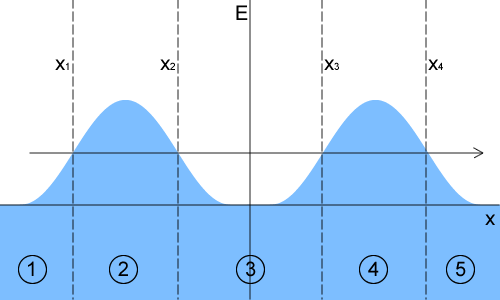
\includegraphics[scale=0.6]{images/s-wkb-double-flat}}
			\caption{Diagram showing a double smooth potential barrier for an arbitrary potentials $V_{1}\left(x\right)$ and $V_{2}\left(x\right)$. The four turning points $x_{1,2,3,4}$ and the five independent barrier regions have been labelled.}
			\label{s-wkb-double-flat}
		\end{figure}
		For a double potential barrier the transmitted wave-function from the first barrier must equal the incoming wave for the second barrier, however the distance between the barriers will create a phase shift. The phase shift can be obtained by matching the incoming and transmitted coefficients. The transmitted wave-function as defined previously:
		\begin{equation}
			y_{t}= q^{-\frac{1}{4}}\left(d_{1}e^{\frac{i}{h}\int_{x_{2}}^{x}\sqrt{q}dx}+d_{2}e^{-\frac{i}{h}\int_{x_{2}}^x \sqrt{q}dx}\right)
		\end{equation}
		must be equal to the incoming wave at the second potential barrier:
		\begin{align}
			y_{i}&= q^{-\frac{1}{4}}\left(a_{3}e^{\frac{i}{h}\int_{x_{3}}^{x}\sqrt{q}dx}+a_{4}e^{-\frac{i}{h}\int_{x_{3}}^x \sqrt{q} dx}\right)\\
			y_{i}&=q^{-\frac{1}{4}}\left(a_{3}e^{-\frac{i}{h}\int_{x_{2}}^{x_{3}}\sqrt{q}dx+\frac{i}{h}\int_{x_{2}}^{x}\sqrt{q}dx}+a_{4}e^{\frac{i}{h}\int_{x_{2}}^{x_{3}}\sqrt{q}dx-\frac{i}{h}\int_{x_{2}}^{x}\sqrt{q}dx}\right)
		\end{align}
		Then the transfer matrix between the two barriers can then be defined as:
		\begin{align}
			\left[\begin{array}{cc}
				d_{1}\\
				d_{2}
			\end{array}\right]
			=
			\left[\begin{array}{cc}
				e^{-\frac{i}{h}P} & 0\\
				0 & e^{\frac{i}{h}P}
			\end{array}\right]
			\left[\begin{array}{cc}
				a_{3}\\
				a_{4}
			\end{array}\right]
		\end{align}
		Where the potentials between the turning points are represented by:
		\begin{equation}
			P=\int_{x_{2}}^{x_{3}}\sqrt{q}dx
		\end{equation}
		With the phase shift between barriers, the total transfer matrix becomes:
		\begin{equation}
			T=T_{2}
			\left[\begin{array}{cc}
				e^{-\frac{i}{h}P} & 0\\
				0 & e^{\frac{i}{h}P}
			\end{array}\right]^{-1}
			T_{1}
		\end{equation}
		Evaluating this with the transfer matrices for each barrier:
		\begin{align}
			T_{11}&=2\cos\left(\frac{P}{h}\right)\left(e^{\frac{Q_{2}}{h}+\frac{Q_{1}}{h}}+\frac{1}{16}e^{-\frac{Q_{2}}{h}-\frac{Q_{1}}{h}}\right)+i\sin\left(\frac{P}{h}\right)\cosh\left(\frac{Q_{2}}{h}-\frac{Q_{1}}{h}\right)\\
			T_{12}&=2i\cos\left(\frac{P}{h}\right)\left(-e^{\frac{Q_{2}}{h}+\frac{Q_{1}}{h}}+\frac{1}{16}e^{-\frac{Q_{2}}{h}-\frac{Q_{1}}{h}}\right)-\sin\left(\frac{P}{h}\right)\sinh\left(\frac{Q_{2}}{h}-\frac{Q_{1}}{h}\right)\\
			T_{21}&=2i\cos\left(\frac{P}{h}\right)\left(e^{\frac{Q_{2}}{h}+\frac{Q_{1}}{h}}-\frac{1}{16}e^{-\frac{Q_{2}}{h}-\frac{Q_{1}}{h}}\right)-\sin\left(\frac{P}{h}\right)\sinh\left(\frac{Q_{2}}{h}-\frac{Q_{1}}{h}\right)\\
			T_{22}&=2\cos\left(\frac{P}{h}\right)\left(e^{\frac{Q_{2}}{h}+\frac{Q_{1}}{h}}+\frac{1}{16}e^{-\frac{Q_{2}}{h}-\frac{Q_{1}}{h}}\right)-i\sin\left(\frac{P}{h}\right)\cosh\left(\frac{Q_{2}}{h}-\frac{Q_{1}}{h}\right)
		\end{align}
		Where each potential is represented by:
		\begin{align}
			Q_{1}=\int_{x_{1}}^{x_{2}}\sqrt{-q}dx
			\hspace{1cm}
			Q_{2}=\int_{x_{3}}^{x_{4}}\sqrt{-q}dx
		\end{align}
		There is a special case when using the Bohr-Sommerfeld quantisation rule and symmetrical barriers:
		\begin{equation}
			P=\pi\left(n+\frac{1}{2}\right)\hspace{1cm}Q_{1}=Q_{2}
		\end{equation}
		which will result in perfect transmission:
		\begin{equation}
			T=\frac{1}{|T_{22}|^{2}}=1
		\end{equation}
%%%%%
%%%%%
%%%%%
%%%%%
%%%%%
	\section{Mathematical Appendix for the WKB Potential Barrier}
		In this section some additional stages in derivations are presented. These stages may be required to fully replicate the results shown, but are too long to include in the main text.
%%%%%
%%%%%
%%%%%
%%%%%
%%%%%
		\subsection{Solutions to Equation (\ref{WKB-w})}
		\label{Appendix-WKB-Solutions}
		The solutions to the equation:
		\begin{equation}
			h^{2}\omega''+\omega\left(\frac{\epsilon^{2}-p_{y}^{2}}{\alpha^{2}}+\frac{ih}{\alpha}\right)=0
		\end{equation}
		are required in the forms:
		\begin{align}
			\omega_{1,3}&=\omega^{+}e^{\frac{i}{h}s}+\omega^{-}e^{-\frac{i}{h}s}\\
			\omega_{2}&=\omega^{+}e^{\frac{1}{h}s}+\omega^{-}e^{-\frac{1}{h}s}
		\end{align}
		For simplicity each term will be evaluated individually, so for $\omega=\omega^{+}e^{\frac{i}{h}s}$ the derivitives:
		\begin{gather}
			\omega'=\frac{i}{h}s'\omega^{+}e^{\frac{i}{h}s}+\omega'^{+}e^{\frac{i}{h}s}\\
			\omega''=\frac{i}{h}s''\omega^{+}e^{\frac{i}{h}s}-\frac{1}{h}s'^{2}\omega^{+}e^{\frac{i}{h}s}+\frac{2i}{h}s'\omega'^{+}e^{\frac{i}{h}s}+\omega''^{+}e^{\frac{i}{h}s}
		\end{gather}
		can be substituted into Equation (\ref{WKB-w}):
		\begin{equation}
			his''\omega^{+}-s'^{2}\omega^{+}+2ihs'\omega'^{+}+h^{2}\omega''^{+}+\frac{\epsilon^{2}-p_{y}^{2}}{\alpha^{2}}\omega^{+}+\frac{ih}{\alpha}\omega^{+}=0
		\end{equation}
		Takeing only $h^{0}$ terms the expression for $s'$ becomes:
		\begin{equation}
			s'=\frac{\sqrt{\epsilon^{2}-p_{y}^{2}}}{\alpha}
		\end{equation}
		Then with only $h$ order terms:
		\begin{equation}
			\frac{2}{\omega^{+}}\omega'^{+}=-\frac{s''}{s'}-\frac{1}{\alpha s'}
		\end{equation}
		With the value of $s'$:
		\begin{equation}
			s''=\frac{\alpha\epsilon-\left(\epsilon^{2}-p_{y}^{2}\right)\alpha'}{\alpha^{2}\sqrt{\epsilon^{2}-p_{y}^{2}}}
		\end{equation}
		Substituting values of $s'$ and $s''$ results in:
		\begin{equation}
			2\frac{\partial}{\partial\epsilon}\ln(\omega^{+})=-\frac{\epsilon}{\epsilon^{2}-p_{y}^{2}}+\frac{\partial}{\partial\epsilon}\ln(\alpha)-\frac{1}{\sqrt{\epsilon^{2}-p_{y}^{2}}}
		\end{equation}
		and integrating:
		\begin{equation}
			2\int_{-p_{y}}^{\epsilon}\frac{\partial}{\partial\epsilon}\ln(\omega^{+})d\epsilon=-\int_{-p_{y}}^{\epsilon}\frac{\epsilon}{\epsilon^{2}-p_{y}^{2}}d\epsilon+\int_{-p_{y}}^{\epsilon}\frac{\partial}{\partial\epsilon}\ln(\alpha) d\epsilon-\int_{-p_{y}}^{\epsilon}\frac{1}{\sqrt{\epsilon^{2}-p_{y}^{2}}}d\epsilon
		\end{equation}
		results in:
		\begin{equation}
			\omega^{+}=\frac{\sqrt{\alpha}}{\left(\epsilon^{2}-p_{y}^{2}\right)^{\frac{1}{4}}}\frac{1}{D^{-}}
		\end{equation}
		where:
		\begin{equation}
			D^{\pm}=\sqrt{\frac{\epsilon+\left(\epsilon^{2}-p_{y}^{2}\right)^{\frac{1}{2}}}{\pm p_{y}}}
		\end{equation}
		The same calculation must then be done for $\omega=\omega^{-}e^{-\frac{i}{h}s}$. With this definition of $\omega$, Equation (\ref{WKB-w}) can be evaluated to:
		\begin{equation}
			his''\omega^{-}-s'^{2}\omega^{-}+2ihs'\omega'^{-}+h^{2}\omega''^{-}+\frac{\epsilon^{2}-p_{y}^{2}}{\alpha^{2}}\omega^{-}-\frac{ih}{\alpha}\omega^{-}=0
		\end{equation}
		Using only the terms of order $h^0$ produces the same result for $s'$ as in the previous case. To find the value of $\omega^{-}$, take only the terms of order $h$:
		\begin{equation}
			2\frac{\partial}{\partial\epsilon}\ln(\omega^{-})=-\frac{s''}{s'}+\frac{1}{\alpha s'}
		\end{equation}
		With the values of $s'$ and $s''$ this relation can be integrated to produce:
		\begin{equation}
			\omega^{-}=\frac{\sqrt{\alpha}}{\left(\epsilon^{2}-p_{y}^{2}\right)^{\frac{1}{4}}}D^{-}
		\end{equation}
		With $\omega=\omega^{+}e^{\frac{1}{h}s}$ in Equation (\ref{WKB-w}) requires the derivities:
		\begin{gather}
			\omega'=\frac{1}{h}s'\omega^{+}e^{\frac{1}{h}s}+\omega'^{+}e^{\frac{1}{h}s}\\
			\omega''=\frac{1}{h}s''\omega^{+}e^{\frac{1}{h}s}+\frac{1}{h^{2}}s'^{2}\omega^{+}e^{\frac{1}{h}s}+\frac{1}{h}2s'\omega'^{+}e^{\frac{1}{h}s}+\omega''^{+}e^{\frac{1}{h}s}
		\end{gather}
		Equation (\ref{WKB-w}) can now be written as:
		\begin{equation}
			s''h\omega^{+}+s'^{2}\omega^{+}+2s'h\omega'^{+}+h^{2}\omega''^{+}+\frac{\epsilon^{2}-p_{y}^{2}}{\alpha^{2}}\omega^{+}+\frac{ih}{\alpha}\omega^{+}=0
		\end{equation}
		With only $h^{0}$ terms, $s'$ becomes:
		\begin{equation}
			s'=\frac{\sqrt{p_{y}^{2}-\epsilon^{2}}}{\alpha}
		\end{equation}
		With only terms of order $h$:
		\begin{equation}
			2\frac{\partial}{\partial\epsilon}\ln(\omega^{+})=-\frac{\partial}{\partial\epsilon}\ln(s')-\frac{i}{\sqrt{p_{y}^{2}-\epsilon^{2}}}
		\end{equation}
		Integrating then results in:
		\begin{equation}
			\omega^{+}=\frac{\sqrt{\alpha}}{\left(p_{y}^{2}-\epsilon^{2}\right)^{\frac{1}{4}}}e^{-\frac{1}{2}i\arcsin\left(\frac{\epsilon}{p_{y}}\right)-\frac{i\pi}{4}}
		\end{equation}
		Finally using $\omega=\omega^{-}e^{-\frac{1}{h}s}$ with Equation (\ref{WKB-w}) produces:
		\begin{equation}
			-s''h\omega^{-}+s'^{2}\omega^{-}-2s'h\omega'^{-}+h^{2}\omega''^{-}+\frac{\epsilon^{2}-p_{y}^{2}}{\alpha^{2}}\omega^{-}+\frac{ih}{\alpha}\omega^{-}=0
		\end{equation}
		The expression produced for $s'$ is identical to that of $\omega^{+}$. Taking only $h$ terms gives the equation:
		\begin{equation}
			2\frac{\omega'^{-}}{\omega^{-}}=-\frac{s''}{s'}+\frac{i}{s'\alpha}
		\end{equation}
		Which when integrated produces:
		\begin{equation}
			\omega^{-}=\frac{\sqrt{\alpha}}{\left(p_{y}^{2}-\epsilon^{2}\right)^{\frac{1}{4}}}e^{\frac{1}{2}i\arcsin\left(\frac{\epsilon}{p_{y}}\right)+\frac{i\pi}{4}}
		\end{equation}
%%%%%
%%%%%
%%%%%
%%%%%
%%%%%
		\subsection{Matching Change of Variables to Solutions of Equation (\ref{WKB-w})}
		\label{Appendix-Matching-Variables}
		The wave-functions produced from the change in variables:
		\begin{equation}
			\omega=\sqrt{\alpha}\left(\frac{u+v}{2}\right)
		\end{equation}
		must match those from the direct solutions from Equation (\ref{WKB-w}). With the trigonometric equations:
		\begin{align}
			\cos^{2}(x)=\frac{1}{1+\tan^{2}(x)}
			\hspace{1cm}
			\cos(x)=\frac{1-\tan^{2}\left(\frac{x}{2}\right)}{1+\tan^{2}\left(\frac{x}{2}\right)}
			\hspace{1cm}
			\sin(x)=\frac{\tan(x)}{\sqrt{1+\tan^{2}(x)}}
		\end{align}
		The grouped terms from the change in variables before and after the barrier can be expressed in the form:
		\begin{align}
			\frac{A^{+}}{P^{+}}&=\frac{1-e^{i\theta}}{\sqrt{1+e^{2i\theta}}}=-\frac{i\sqrt{2}\sin\left(\frac{\theta}{2}\right)}{\sqrt{\cos(\theta)}}=-\sqrt{\frac{2}{1-\cot^{2}\left(\frac{\theta}{2}\right)}}\\
			\frac{A^{-}}{P^{-}}&=\frac{1+e^{-i\theta}}{\sqrt{1+e^{-2i\theta}}}=\frac{\sqrt{2}\cos\left(\frac{\theta}{2}\right)}{\sqrt{\cos(\theta)}}=\sqrt{\frac{2}{1-\tan^{2}\left(\frac{\theta}{2}\right)}}
		\end{align}
		Then with the additional identities:
		\begin{align}
			\frac{q+p_{y}}{-\epsilon}=\tan(\alpha)
			\hspace{1cm}
			\frac{-q+p_{y}}{-\epsilon}=\tan(-\alpha)
			\hspace{1cm}
			\tan^{2}(x)-1=-\frac{\cos(2x)}{\cos^{2}(x)}
		\end{align}
		The terms for use inside the barrier can be converted to:
		\begin{equation}
			\frac{B^{+}}{Q^{+}}=\frac{1+i\tan(\alpha)}{\sqrt{-\frac{\cos(2\alpha)}{\cos^{2}(\alpha)}}}=\frac{\cos(\alpha)+i\sin(\alpha)}{\sqrt{-\cos(2\alpha)}}=\frac{e^{i\alpha}}{\sqrt{-\cos(2\alpha)}}
		\end{equation}
		\begin{equation}
			\frac{B^{-}}{Q^{-}}=\frac{1+i\tan(-\alpha)}{\sqrt{-\frac{\cos(2\alpha)}{\cos^{2}(\alpha)}}}=\frac{\cos(-\alpha)+i\sin(-\alpha)}{\sqrt{-\cos(2\alpha)}}=\frac{e^{-i\alpha}}{\sqrt{-\cos(2\alpha)}}
		\end{equation}
		The grouped terms in the direct solutions to Equation (\ref{WKB-w}) must now be shown in the same form. With the additional equations:
		\begin{align}
			\tan(\theta)=\frac{p_{y}}{p_{x}}=\frac{p_{y}}{\sqrt{\epsilon^{2}-p_{y}^{2}}}
			\hspace{1cm}
			\frac{1}{\tan^{2}(\theta)}=\frac{\epsilon}{p_{y}^{2}}-1=\frac{1}{\sin^{2}(\theta)}-1
			\hspace{1cm}
			\frac{1}{\sin(\theta)}=\frac{\epsilon}{p_{y}}
		\end{align}		
		\begin{align}
			\sin(x)=\frac{2\tan\left(\frac{x}{2}\right)}{\tan^{2}\left(\frac{x}{2}\right)+1}
			\hspace{1cm}
			\cos(x)=\frac{1-\tan^{2}\left(\frac{x}{2}\right)}{1+\tan^{2}\left(\frac{x}{2}\right)}
			\hspace{1cm}
			\cot(x)=\frac{1-\tan^{2}\left(\frac{x}{2}\right)}{2\tan\left(\frac{x}{2}\right)}
		\end{align}
		\begin{align}
			D^{\pm}=\sqrt{\frac{\epsilon+\sqrt{\epsilon^{2}-p_{y}^{2}}}{-p_{y}}}
		\end{align}
		The grouped terms from the solutions of Equation (\ref{WKB-w}) can be expressed as:
		\begin{align}
			\frac{\sqrt{p_{y}}}{\left(\epsilon^{2}-p_{y}^{2}\right)^{\frac{1}{4}}}\frac{1}{D^{-}}&=\sqrt{-\frac{\tan(\theta)}{\frac{1}{\sin(\theta)}+\cot(\theta)}}=\sqrt{\frac{2}{1-\cot^{2}\left(\frac{\theta}{2}\right)}}
			\\
			\frac{\sqrt{p_{y}}}{\left(\epsilon^{2}-p_{y}^{2}\right)^{\frac{1}{4}}}D^{-}&=\sqrt{-\tan(\theta)\left(\frac{1}{\sin(\theta)}+\cot(\theta)\right)}=\sqrt{-\frac{2}{1-\tan^{2}\left(\frac{\theta}{2}\right)}}
			\\
			\frac{\sqrt{p_{y}}}{\left(\epsilon^{2}-p_{y}^{2}\right)^{\frac{1}{4}}}\frac{1}{D^{+}}&=\sqrt{-\frac{\tan(\theta)}{\frac{1}{\sin(\theta)}+\cot(\theta)}}=\sqrt{-\frac{2}{1-\cot^{2}\left(\frac{\theta}{2}\right)}}
			\\
			\frac{\sqrt{p_{y}}}{\left(\epsilon^{2}-p_{y}^{2}\right)^{\frac{1}{4}}}D^{+}&=\sqrt{-\tan(\theta)\left(\frac{1}{\sin(\theta)}+\cot(\theta)\right)}=\sqrt{\frac{2}{1-\tan^{2}\left(\frac{\theta}{2}\right)}}
		\end{align}
		Then the solutions inside the barrier can be converted with the definition:
		\begin{align}
			\frac{\epsilon}{p_{y}}=\sin(2\alpha)
			\hspace{1cm}
			\sin^{2}(x)=1-\cos^{2}(x)
			\hspace{1cm}\sqrt{\frac{p_{y}^{2}-\epsilon^{2}}{p_{y}^{2}}}=\cos(2\alpha)
		\end{align}
		\begin{equation}
			\frac{\sqrt{p_{y}}}{\left(p_{y}^{2}-\epsilon^{2}\right)^{\frac{1}{4}}}e^{\frac{i}{2}\arcsin\left(\frac{\epsilon}{p_{y}}\right)}=\frac{e^{i\alpha}}{\sqrt{\cos(2\alpha)}}
		\end{equation}
		\begin{equation}
			\frac{\sqrt{p_{y}}}{\left(p_{y}^{2}-\epsilon^{2}\right)^{\frac{1}{4}}}e^{-\frac{i}{2}\arcsin\left(\frac{\epsilon}{p_{y}}\right)}=\frac{e^{-i\alpha}}{\sqrt{\cos(2\alpha)}}
		\end{equation}
%%%%%
%%%%%
%%%%%
%%%%%
%%%%%
		\subsection{Matching Solutions of Equation (\ref{WKB-w}) to Schr{\" o}dinger Solutions}
		\label{Appendix-Matching-Solutions}
		Here it will be shown how the solutions to Equation (\ref{WKB-w}) are comparable to the WKB solutions for the Schr{\" o}dinger equation. The integral from Equation (\ref{omega-final}) shall be defined as:
		\begin{equation}
			I=\int^{\epsilon}_{-p_{y}}\frac{\sqrt{\epsilon^{2}-p_{y}^{2}}}{\alpha}d\epsilon
		\end{equation}
		The change in variable:
		\begin{equation}
			y^{2}=\epsilon^{2}+mh\alpha
		\end{equation}
		will now be introduced, this change in variable includes a small variation. To convert the integral $I$ to terms of $y$, an expression for $d\epsilon /dy$ is required.
		\begin{equation}
			ydy=\left(2\epsilon+mh\alpha '\right) d\epsilon
		\end{equation}
		With a further substitution of $\epsilon = \sqrt{y^{2}-mh\alpha}$ this can take the form:
		\begin{equation}
			2\frac{d\epsilon}{dy}=\frac{1}{\sqrt{1-\frac{mh\alpha}{y^{2}}}+\frac{mh\alpha '}{2y}}
		\end{equation}
		A Taylor expansion of $\sqrt{1-\frac{mh\alpha}{y^{2}}}$ at $\frac{mh\alpha}{y^{2}}=0$ produces:
		\begin{equation}
			2\frac{d\epsilon}{dy}=\frac{1}{1-\frac{mh\alpha}{2y^{2}}+\frac{mh\alpha '}{2y}}
		\end{equation}
		A further Taylor expansion results in:
		\begin{equation}
			2\frac{d\epsilon}{dy}=1+\frac{mh\alpha}{2y^{2}}-\frac{mh\alpha '}{2y}
		\end{equation}
		Next the function $\alpha\left(\epsilon\right)$ must be converted to be a function of $y$:
		\begin{equation}
			\alpha\left(\epsilon\right)=\alpha\left(\epsilon\left(y\right)\right)=\alpha\left(\sqrt{y^{2}-mh\alpha}\right)
		\end{equation}
		The Laurent series of $\sqrt{y^{2}-mh\alpha}$ at $y=\infty$ results in:
		\begin{equation}
			\alpha\left(\epsilon\right)=\alpha\left(y-\frac{mh\alpha}{2y}\right)
		\end{equation}
		Then the Taylor expansion at $mh\alpha / 2y=0$ shows:
		\begin{equation}
			\alpha\left(\epsilon\right)=\alpha\left(y\right)-\frac{mh\alpha}{2y}\alpha'
		\end{equation}
		A final Taylor expansion around $mh\alpha'/2y=0$ shows that:
		\begin{equation}
			\frac{1}{\alpha\left(\epsilon\right)}=\frac{1}{\alpha\left(y\right)}\left(1+\frac{mh\alpha'}{2y}\right)
		\end{equation}
		With these definitions the integral $I$ can be expressed as:
		\begin{equation}
			I=\int^{\epsilon}_{-p_{y}}\frac{\sqrt{\epsilon^{2}-p_{y}^{2}}}{\alpha\left(\epsilon\right)}d\epsilon=\int^{y}_{-p_{y}}\frac{\sqrt{y^{2}-p_{y}^{2}}}{\alpha\left(y\right)}\left(1+\frac{hm\alpha '}{2y}\right)\left(1+\frac{mh\alpha}{2y^{2}}-\frac{mh\alpha '}{2y}\right)dy
		\end{equation}
		Evaluating the brackets, and removing terms of order $h^{2}$:
		\begin{equation}
			I=\int^{\epsilon}_{-p_{y}}\frac{\sqrt{\epsilon^{2}-p_{y}^{2}}}{\alpha\left(\epsilon\right)}d\epsilon=\int^{y}_{-p_{y}}\frac{\sqrt{y^{2}-p_{y}^{2}}}{\alpha}dy+\frac{mh}{2}\int^{y}_{-p_{y}}\frac{\sqrt{y^{2}-p_{y}^{2}}}{y^{2}}dy
		\end{equation}
		Introducing a small pertubation to $y$ changes the function $f\left(y\right)=f\left(y+\Delta y\right)$, this is required in a manor that $\Delta \gg h$. An expansion of this produces $f\left(y+\Delta y\right)=f\left(y\right)+\Delta y f'\left(y\right)$. This allows the integral:
		\begin{equation}
			\frac{mh}{2}\int^{y}_{-p_{y}}\frac{\sqrt{y^{2}-p_{y}^{2}}}{y^{2}}dy=\frac{mh}{2}\int^{y}_{-p_{y}}\frac{\sqrt{y^{2}-p_{y}^{2}}}{y^{2}}dy+\frac{mh}{2}\frac{\sqrt{y^{2}-p_{y}^{2}}}{y}
		\end{equation}
		To the leading order, $y=\epsilon$, therefore the integral can be evaluated to:
		\begin{equation}
			\int^{\epsilon}_{-p_{y}}\frac{\sqrt{y^{2}-p_{y}^{2}}}{y^{2}}dy=\ln\left(\frac{\sqrt{\epsilon^{2}+p_{y}^{2}}+\epsilon}{-p_{y}}\right)-\frac{\sqrt{\epsilon^{2}+p_{y}^{2}}}{\epsilon}
		\end{equation}
		These pertubations result in:
		\begin{equation}
			\int^{\epsilon}_{-p_{y}}\frac{\sqrt{\epsilon^{2}-p_{y}^{2}}}{\alpha}d\epsilon=\int^{\epsilon}_{-p_{y}}\frac{\sqrt{\epsilon^{2}-p_{y}^{2}}}{\alpha}d\epsilon+\frac{h}{2}\ln\left(\frac{\sqrt{\epsilon^{2}+p_{y}^{2}}+\epsilon}{-p_{y}}\right)
		\end{equation}
		For the wave-function before the barrier, $-p_{y}$ is larger then $\epsilon$, therefore:
		\begin{equation}
			\int^{-p_{y}}_{\epsilon}\frac{\sqrt{\epsilon^{2}-p_{y}^{2}}}{\alpha}d\epsilon=-\int^{\epsilon}_{-p_{y}}\frac{\sqrt{\epsilon^{2}-p_{y}^{2}}}{\alpha}d\epsilon-\frac{h}{2}\ln\left(\frac{\sqrt{\epsilon^{2}+p_{y}^{2}}+\epsilon}{-p_{y}}\right)
		\end{equation}
		and the wave-function component before the first turning point becomes:
		\begin{equation}
			\frac{\sqrt{\alpha}}{\left(\epsilon^{2}-p_{y}^{2}\right)^{\frac{1}{4}}}a_{1}\frac{1}{D^{-}}e^{\frac{i}{h}\int^{-p_{y}}_{\epsilon}\frac{\sqrt{\epsilon^{2}-p_{y}^{2}}}{\alpha}d\epsilon}=\frac{1}{q^{\frac{1}{4}}}\bar{a}_{1}e^{\frac{i}{h}\int_{x}^{x_{1}} \sqrt{q} dx}
		\end{equation}
		with:
		\begin{equation}
			q=\sqrt{\frac{\epsilon^{2}-p_{y}^{2}}{\alpha^{2}}}
			\hspace{1cm}
			D^{\pm}=\sqrt{\frac{\epsilon+\sqrt{\epsilon^{2}-p_{y}^{2}}}{\pm p_{y}}}
		\end{equation}
		Similarly with the wave-function components:
		\begin{align}
			\frac{\sqrt{\alpha}}{\left(\epsilon^{2}-p_{y}^{2}\right)^{\frac{1}{4}}}a_{2}D^{-}e^{-\frac{i}{h}\int^{-p_{y}}_{\epsilon}\frac{\sqrt{\epsilon^{2}-p_{y}^{2}}}{\alpha}d\epsilon}&=\frac{1}{q^{\frac{1}{4}}}\bar{a}_{2}e^{-\frac{i}{h}\int_{x}^{x_{1}} \sqrt{q} dx}\\
			\frac{\sqrt{\alpha}}{\left(\epsilon^{2}-p_{y}^{2}\right)^{\frac{1}{4}}}d_{1}\frac{1}{D^{+}}e^{\frac{i}{h}\int^{\epsilon}_{p_{y}}\frac{\sqrt{\epsilon^{2}-p_{y}^{2}}}{\alpha}d\epsilon}&=\frac{1}{q^{\frac{1}{4}}}\bar{d}_{2}e^{\frac{i}{h}\int_{x_{2}}^x \sqrt{q} dx}\\
			\frac{\sqrt{\alpha}}{\left(\epsilon^{2}-p_{y}^{2}\right)^{\frac{1}{4}}}d_{2}D^{+}e^{-\frac{i}{h}\int^{\epsilon}_{p_{y}}\frac{\sqrt{\epsilon^{2}-p_{y}^{2}}}{\alpha}d\epsilon}&=\frac{1}{q^{\frac{1}{4}}}\bar{d}_{1}e^{-\frac{i}{h}\int_{x_{2}}^x \sqrt{q} dx}
		\end{align}
		For the case inside the barriers the additional terms included in the $\omega$ functions may be absorbed into the constants.
%\end{document}